
\begin{table*}[t]
\centering
\small
\setlength{\tabcolsep}{6pt}
\renewcommand{\arraystretch}{1.15}

\caption{
      \textbf{Security Property Satisfaction of Third‑Party Online Payment Protocols.}
      Each protocol is evaluated under three channel security assumptions. 
      IA-O1/O2, IA-UA, IA-R1/R2 denote the security properties defined in Section~\ref{sec:security_properties}.
      \textcolor{green}{\ding{51}} indicates that the security property is satisfied, while \textcolor{red}{\ding{55}} indicates a violation.
      Time reports the total analysis time.
    }
\label{tab:lemma-results}

\begin{tabularx}{\textwidth}{XXXXcccccr}
\toprule

\textbf{Provider} & \textbf{Scenario} & \textbf{Model} & \textbf{Assumption} & \textbf{\; IA-O1 \;} & \textbf{\; IA-O2 \;} & \textbf{\; IA-UA \;} & \textbf{\; IA-R1 \;} & \textbf{\; IA-R2 \;} & \textbf{Time (s)}\\

\midrule

Alipay & In-App & A & Base & \textcolor{red}{\ding{55}} & \textcolor{red}{\ding{55}} & \textcolor{green}{\ding{51}} & \textcolor{green}{\ding{51}} & \textcolor{green}{\ding{51}} & 265.8 \\
Alipay & Mobile-Web & A & Base & \textcolor{red}{\ding{55}} & \textcolor{red}{\ding{55}} & \textcolor{green}{\ding{51}} & \textcolor{green}{\ding{51}} & \textcolor{green}{\ding{51}} & 266.22 \\
Alipay & QR-Code & B & Base & \textcolor{green}{\ding{51}} & \textcolor{red}{\ding{55}} & \textcolor{green}{\ding{51}} & \textcolor{green}{\ding{51}} & \textcolor{green}{\ding{51}} & 606.59 \\
WeChatPay & In-App & B & Base & \textcolor{green}{\ding{51}} & \textcolor{red}{\ding{55}} & \textcolor{green}{\ding{51}} & \textcolor{green}{\ding{51}} & \textcolor{green}{\ding{51}} & 562.21 \\
WeChatPay & Mobile-Web & B & Base & \textcolor{green}{\ding{51}} & \textcolor{red}{\ding{55}} & \textcolor{green}{\ding{51}} & \textcolor{green}{\ding{51}} & \textcolor{green}{\ding{51}} & 88.18 \\
WeChatPay & QR-Code & B & Base & \textcolor{green}{\ding{51}} & \textcolor{red}{\ding{55}} & \textcolor{green}{\ding{51}} & \textcolor{green}{\ding{51}} & \textcolor{green}{\ding{51}} & 123.89 \\
\midrule
Alipay & In-App & A & SecureMS & \textcolor{red}{\ding{55}} & \textcolor{red}{\ding{55}} & \textcolor{green}{\ding{51}} & \textcolor{green}{\ding{51}} & \textcolor{green}{\ding{51}} & 13.94 \\
Alipay & Mobile-Web & A & SecureMS & \textcolor{red}{\ding{55}} & \textcolor{red}{\ding{55}} & \textcolor{green}{\ding{51}} & \textcolor{green}{\ding{51}} & \textcolor{green}{\ding{51}} & 14.39 \\
Alipay & QR-Code & B & SecureMS & \textcolor{green}{\ding{51}} & \textcolor{red}{\ding{55}} & \textcolor{green}{\ding{51}} & \textcolor{green}{\ding{51}} & \textcolor{green}{\ding{51}} & 73.57 \\
WeChatPay & In-App & B & SecureMS & \textcolor{green}{\ding{51}} & \textcolor{red}{\ding{55}} & \textcolor{green}{\ding{51}} & \textcolor{green}{\ding{51}} & \textcolor{green}{\ding{51}} & 19.96 \\
WeChatPay & Mobile-Web & B & SecureMS & \textcolor{green}{\ding{51}} & \textcolor{red}{\ding{55}} & \textcolor{green}{\ding{51}} & \textcolor{green}{\ding{51}} & \textcolor{green}{\ding{51}} & 7.73 \\
WeChatPay & QR-Code & B & SecureMS & \textcolor{green}{\ding{51}} & \textcolor{red}{\ding{55}} & \textcolor{green}{\ding{51}} & \textcolor{green}{\ding{51}} & \textcolor{green}{\ding{51}} & 7.22 \\
\midrule
Alipay & In-App & A & SecurePS & \textcolor{red}{\ding{55}} & \textcolor{red}{\ding{55}} & \textcolor{green}{\ding{51}} & \textcolor{green}{\ding{51}} & \textcolor{green}{\ding{51}} & 19.55 \\
Alipay & Mobile-Web & A & SecurePS & \textcolor{red}{\ding{55}} & \textcolor{red}{\ding{55}} & \textcolor{green}{\ding{51}} & \textcolor{green}{\ding{51}} & \textcolor{green}{\ding{51}} & 18.2 \\
Alipay & QR-Code & B & SecurePS & \textcolor{green}{\ding{51}} & \textcolor{red}{\ding{55}} & \textcolor{green}{\ding{51}} & \textcolor{green}{\ding{51}} & \textcolor{green}{\ding{51}} & 155.14 \\
WeChatPay & In-App & B & SecurePS & \textcolor{green}{\ding{51}} & \textcolor{red}{\ding{55}} & \textcolor{green}{\ding{51}} & \textcolor{green}{\ding{51}} & \textcolor{green}{\ding{51}} & 159.02 \\
WeChatPay & Mobile-Web & B & SecurePS & \textcolor{green}{\ding{51}} & \textcolor{red}{\ding{55}} & \textcolor{green}{\ding{51}} & \textcolor{green}{\ding{51}} & \textcolor{green}{\ding{51}} & 20.66 \\
WeChatPay & QR-Code & B & SecurePS & \textcolor{green}{\ding{51}} & \textcolor{red}{\ding{55}} & \textcolor{green}{\ding{51}} & \textcolor{green}{\ding{51}} & \textcolor{green}{\ding{51}} & 26.77 \\

\bottomrule
\end{tabularx}
\end{table*}

%-------------------------------------------------------------------------------
\section{Analysis Results}  \label{sec:results}
%-------------------------------------------------------------------------------

We conducted a comprehensive automated security analysis of three payment scenarios of WeChat Pay and Alipay under three channel security assumptions using Tamarin Prover version~1.10.0 on a server equipped with a 24-core, 32-thread Intel Core i9-14900K CPU and 192\,GB of memory, running Ubuntu~24.04~LTS. 
This section presents the verification results in detail. 

\subsection{Results}

Table~\ref{tab:lemma-results} summarizes our analysis results.
We find that two protocols following Payment Model~A also fail to satisfy the IA-O1 property under all three channel assumptions. 
When it comes to IA-O2 , regardless of whether they belong to Payment Model~A or Payment Model~B, fail to satisfy the IA-O2 property.
The corresponding counterexample traces reveal the order tampering attack and its variants.

\subsection{Order Tampering Attack}

In an Order Tampering Attack, the attacker misleads both the user and the merchant into becoming confused about the order, thereby causing the user to authorize an incorrect order.
This attack was first identified by \cite{Yang2017FlawedImplementations} in the In-App payment scenario.
Our model-based analysis shows that Order Tampering Attacks are prevalent, can be extended to other payment scenarios, and admit distinct variants.

\begin{figure}[t]
  \centering
  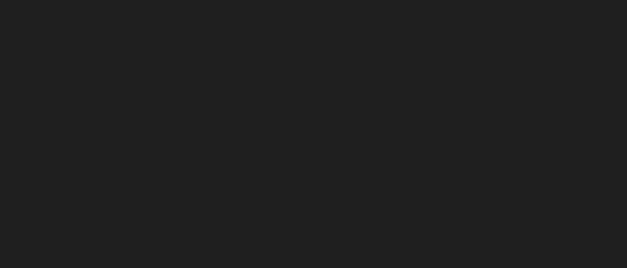
\includegraphics[width=\linewidth]{img/black.png}
  \caption{Order Tampering Attack Variant 1}
  \label{fig:order_tampering_variant_1}
\end{figure}

\begin{figure}[t]
  \centering
  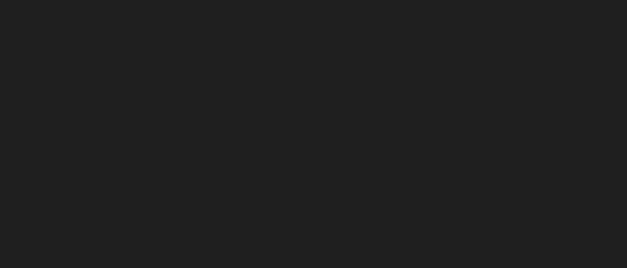
\includegraphics[width=\linewidth]{img/black.png}
  \caption{Order Tampering Attack Variant 2}
  \label{fig:order_tampering_variant_2}
\end{figure}

There are two variants of the Order Tampering Attack, as illustrated in Figures~\ref{fig:order_tampering_variant_1} and~\ref{fig:order_tampering_variant_2}.
The main difference between these two variants lies in the communication channel over which the attacker tampers with the order.
In Variant~1, the attacker tampers with the communication channel between \emph{MF} and \emph{MS}, thereby causing \emph{U} to ultimately authorize an order specified by the attacker.
In Variant~2, the order is tampered with by the attacker on the communication channel between \emph{MF} and \emph{PS}.
We identify a widely prevalent vulnerability that can be exploited to mount the Variant~2 Order Tampering Attack, which will be discussed in detail in Section~\ref{sec:real_world}.
